% !TEX encoding = UTF-8
% !TEX TS-program = pdflatex
% !TEX root = ../tesi.tex

%**************************************************************
\chapter{Study case: AWS EC2 resource generation with Pulumi}
\label{cap:case-study}
%**************************************************************

\intro{Generation of AWS EC2 resources with Pulumi to compare how various languages supported by Pulumi will differ in the infrastructure resources declaration}\\

%**************************************************************
\section{Amazon Web Services}
AWS is a wide collection of services with many different purposes and characteristics including compute, storage, databases, analytics, networking, mobile, developer tools, management tools, IoT, security, and enterprise applications: on-demand, available in seconds, with pay-as-you-go pricing.
Anyway, for the purpose of the thesis we'll focus only on the EC2 module.

\subsection{AWS's EC2 module}
EC2 provides scalable computing capacity in the Amazon Web Services (AWS) Cloud.
Amazon EC2 eliminates the need to invest in hardware up front, so that the development and deployment of the applications is faster.
Such a characteristics is a perfect fit for an IaC scenario.

\section{Case study infrastructure overview}
For the thesis, only few components of the vast EC2 module have been selected to create a working infrastructure.\\
The infrastructure

\subsection{Components of the infrastructure}
The infrastructure we created for the case study of the thesis is an AWS EC2 \gls{VPC} hosting 3 private \gls{subnet}s, 3 public subnets, an \gls{internet gateway} to let the public subnets connect to the internet and a \gls{routing table} to map the public subnets to the internet gateway.
The architecture will look like the following:
\begin{center}
  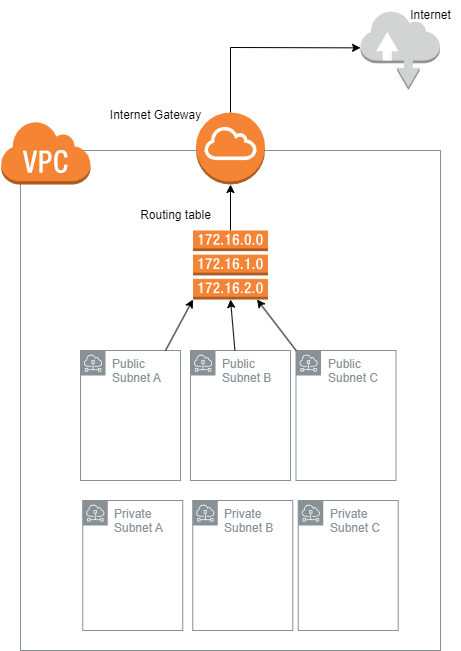
\includegraphics[width=1\columnwidth]{case_study/vpc_diagram} 
  \captionof{figure}{Infrastrutcture Architecture}
\end{center}\mbox{}\\
AWS is divided into regions, like us-east-1, eu-central-1, eu-south-1, etc.
For the purpose of our thesis eu-south-1 as a region has been chosen.
The servers of such a region are located in Milan.
Each region can have multiple availability zones, eu-south-1 has 3 different availability zones, and because of this we chose to create 3 couples of public/private subnets (A-A, B-B, C-C).
One couple on each availability zone.
The purpose of the availability zones is mainly for robustness.
If an availability zone becomes temporary unavailable, we can rely on the others to keep our services up.


\subsubsection{VPC}
The VPC is our "container" for all the other infrastructure resources.
We'll define within it the subnets, the internet gateway and the outing table.\\
The most important setting of our AWS EC2 VPC is the CIDR (Classless Inter-Domain Routing) block.
It represents the range of private IP addresses that the VPC can use to create and manage resources within the VPC.
\paragraph{CIDR}
The CIDR block is used to define the range of IP addresses that the VPC can use.
In our case the CIDR block is 10.136.0.0/24, which means that the VPC has access to all IP addresses from 10.136.0.0 to 10.136.0.255.
The 24 in the CIDR block is the prefix length, aka the subnet mask, that is used to identify the VPC.
The remaining 8 bits of the IP address will be used to identify the hosts in the VPC.\\
We'll assign a name as well to our VPC so that will be easier to recognize it when we'll inspect the AWS Management Console, that is the GUI version of the AWS CLI.

%val pvtSubnetsCidrs: List[String] = List("10.136.0.0/27", "10.136.0.32/27", "10.136.0.64/27")
%val pubSubnetsCidrs: List[String] = List("10.136.0.96/27", "10.136.0.128/27", "10.136.0.160/27")

\subsubsection{Subnet}
The subnets will require the ID of the VPC and the CIDR block that defines their IP scope.
For the subnets we'll use the following CIDR blocks:
\begin{itemize}
  \item Private Subnet A: 10.136.0.0/27
  \item Private Subnet B: 10.136.0.32/27
  \item Private Subnet C: 10.136.0.64/27
  \item Public Subnet A: 10.136.0.96/27
  \item Public Subnet B: 10.136.0.128/27
  \item Public Subnet C: 10.136.0.160/27
\end{itemize}
3 of the 8 bits left out for the hosts identification have been used to identify the subnets.
In fact we shall notice that now the subnet mask is not 24 anymore, but 27.
Hence, we are left with 5 bits to identify the hosts within each subnet, giving us 32 possible IPs.
From such IPs 2 are reserved for the network address and the broadcast address, so we have 30 possible IPs.
We won't discuss this topic any further since it isn't essential for the final objective of the thesis.\\
Moreover, we'll define also the availability zone for each subnet.


\subsubsection{InternetGateway}
The definition of the internet gateway is actually quite straight forward.
The mandatory parameter to assign is the ID of the VPC.

\subsubsection{RouteTable}
\label{sssec:routetable}
The definition of a route table is required in order to bind the public subnets to the internet gateway, so that they can send and receive data over the internet.\\
Here, along with the VPC ID, we assign the routes of such routing table.
In order to do this we have to provide a CIDR and a target resource to which the packet will be forwarded to, that can be a subnet or the internet gateway in our case.
The internet gateway is mapped with the CIDR block 0.0.0.0/0.
Obviously also the ID of the internet gateway is required in order to bind it to the routing table.\\
In a nutshell this means that every packet not directed to a host within the VPC will be routed to the internet gateway and then to the internet.\\
The association of the public subnets to the routing table will be achieved using the \textit{route table association} resource.
Such a resource will require us to provide the id of the subnet and the id of the routing table to establish a connection.
The private subnets will not be associated to such a routing table, since we want to keep them private.
Differently, without explicitly associating them to a given routing table, AWS will automatically associate them to a default routing table that, being not bound to an internet gateway, will keep them private.\\


\section{Typescript implementation of the case study}
\label{sec:typescript-impl}
The first version of the implementation of the previously defined architecture is written using the Typescript APIs of Pulumi.
The structure of the project, and this holds for the Java and Scala version as well, is trivial.
We have a simple \texttt{index.ts} file that defines the entry point for our typescript project, and it is just a couple of lines long:
\begin{lstlisting}[numbers=left, numberstyle=\tiny, numbersep=-5pt, stepnumber=1]
  import { VPC } from './VPC/VPC';

  const vpc = new MyVPC("Custom VPC");
\end{lstlisting}\mbox{}\\
The interesting part relies on the \texttt{MyVPC} class.
Such a class extends the \texttt{ComponentResource} class of Pulumi.
In our typescript implementation, we use the constructor of the user-defined \texttt{MyVPC} class to call all the class methods that are responsible for the creation of the resources.
But this is just mentioned since the interesting part of the code are the actual methods that are responsible for the creation of the resources.

\subsection{VPC resource creation}
The code to the VPC resource creation API of Pulumi is done in this method of the \texttt{MyVPC} class:
\begin{lstlisting}[numbers=left, numberstyle=\tiny, numbersep=-5pt, stepnumber=1]
  protected createVPC() {
    this.vpc = new Vpc("vpc\_res", {
      cidrBlock: "10.136.0.0/24",
      tags: {
        Name: "myVPC-typescript",
      },
    },
    {
      parent: this,
    });
  }
\end{lstlisting}\mbox{}\\
\texttt{vpc\_res} is the name that will be given by Pulumi at this resource once on the stack.
We can notice how the various parameters are given in a declarative style within the curly brackets.
Such a syntax is syntactic sugar for a Map definition.\\
At line 8 the parent of this resource is set.
With this specification, we are telling to the stack of Pulumi that the vpc resource \texttt{vpc\_res} that we are creating is a child resource of the VPC resource identified by the \texttt{MyVPC} class.

\subsection{Internet gateway creation}
To create the internet gateway resource we can use the following code:
\begin{lstlisting}[numbers=left, numberstyle=\tiny, numbersep=-5pt, stepnumber=1]
  protected createIGW(){
    this.gw = new InternetGateway("gw", {
      vpcId: this.vpc?.id,
      tags: {
          Name: "myIGW-typescript",
      },
    },
    {
      parent: this.vpc,
    });
  }
\end{lstlisting}\mbox{}\\
It is really simple since it requires just the ID of the VPC in which it has to be created and optionally a name and a parent for the Pulumi's stack representation.


\subsection{Subnets creation}
To create the private and the public subnets we require a more complex logic.
The function that has been used is \texttt{protected createAZsSubnets(isPvt: Boolean)}.
It is called twice, once with a true value to create the private subnets, and another one with false to instantiate the public ones (and connect them to the routing table bound with the internet gateway).\\
In the body of the function, first we want to get all the availability zones present in the AWS region we are working on.
To achieve this, we will use such a function \texttt{this.availableZones = aws.getAvailabilityZonesOutput()}.\\
Second, we want to create both a private and public subnet in each availability zone acquired with the aforementioned method.
The \texttt{pulumi.all} function, in combination with the \texttt{apply} function will help us in achieving such a goal.\\

\subsubsection{pulumi.all}
\texttt{pulumi.all} is a utility function in Pulumi that allows you to combine multiple Outputs into a single Output that resolves to an array of the resolved values of each Output.
So if we consider the following code:
\begin{lstlisting}[numbers=left, numberstyle=\tiny, numbersep=-5pt, stepnumber=1]
  pulumi.all([this.availableZones.names, this.vpc!.id])
\end{lstlisting}\mbox{}\\
Such a call returns us an \texttt{Output<[string[], string]>}.
The array of strings is the list of the availability zones names, while the second string represents the ID of our VPC on AWS EC2.
Now we have a new Output type that is more suitable to create the subnets based on our VPC ID, because the function apply is letting us "open" an \texttt{Output} value and access its content.

\subsubsection{.apply}
Lets extend our code in this way:
\begin{lstlisting}[numbers=left, numberstyle=\tiny, numbersep=-5pt, stepnumber=1]
  pulumi.all([this.availableZones.names, this.vpc!.id]).apply(([azNames, vpcId]) => {
    // lambda's body to create the subnets here
  })
\end{lstlisting}\mbox{}\\
The apply function is letting us access \texttt{Output<[string[], string]>} and apply some logic on the inner values.\\

\paragraph{The apply's lambda}
Now that we have the access to the list of availability zones and the VPC ID, we can iterate over the availability zones and create the subnets for our VPC.
Here is the complete code of the function:
\begin{lstlisting}[numbers=left, numberstyle=\tiny, numbersep=-5pt, stepnumber=1]
  protected createAZsSubnets(isPvt: Boolean){
    this.availableZones = aws.getAvailabilityZonesOutput()
    pulumi.all([this.availableZones.names, this.vpc!.id]).apply(([azNames, vpcId]) => {
      let i = 0
      let listToPushInto: Subnet[] = Array<aws.ec2.Subnet>()
      azNames.forEach(azName => {
        let compName = azName + (isPvt ? "-pvt" : "-pub") + "-subnet-typescript"
        listToPushInto.push(new Subnet(compName, {
          vpcId: vpcId,
          availabilityZone: azName,
          cidrBlock: isPvt ? this.pvtSubnetsCidrs[i] : this.pubSubnetsCidrs[i],
          tags: {
            Name: compName,
          },
        },
        {
          parent: this.vpc
        }
        ));
        i++;
      });
      if(!isPvt){
        this.pubSubNets = listToPushInto
        // attaching the route table to the pub sub nets
        this.attachRouteTableToPubSubnets()
      }
      else
        this.prvSubNets = listToPushInto
    });
  }
\end{lstlisting}\mbox{}\\
In the code we instantiate private or public public subnets basing on the \texttt{isPvt} passed in the \texttt{createAZsSubnets}.
We can notice that for the creation of a subnet we pass arguments such as \texttt{vpcId}, the availability zone name, the CIDR block, and a name (that is a tag) to better identify it on the stack.\\
Each newly created subnet is then pushed into the class field \texttt{this.prvSubNets} or \texttt{this.pubSubNets} (that are arrays of subnets), basing on the nature of the subnet.
The \texttt{this.pubSubNets} will be used by the \texttt{this.attachRouteTableToPubSubnets()} function to bind the public subnets to the internet gateway through the routing table.\\
The crucial point here is that in order to bind the public subnets to the routing table, we must call \texttt{this.attachRouteTableToPubSubnets()} as the last step in our \texttt{pulumi.all} function call.
This ensures that we have all the necessary subnets to make the binding, since the call will be done at the completion of the creation of the subnets.

\subsection{Routing table creation}
This is the code to create the routing table resource:
\begin{lstlisting}[numbers=left, numberstyle=\tiny, numbersep=-5pt, stepnumber=1]
  protected createRouteTable() {
    this.routeTable = new RouteTable("example", {
      vpcId: this.vpc!.id,
      routes: [
          {
              cidrBlock: "0.0.0.0/0",
              gatewayId: this.gw!.id,
          },
      ],
      tags: {
          Name: "myRouteTable-typescript",
      },
  },
  {
    parent: this.vpc,
  });
  }
\end{lstlisting}\mbox{}\\
On top of the classic VPC ID we are assigning here the routes.
As we mentioned before in the \hyperref[sssec:routetable]{Routetable} paragraph, we are defining the route with CIDR 0.0.0.0/0 to redirect all the packets coming from the public subnets, and not having as destination an IP internal at our VPC, to the internet gateway.\\
We are also giving a name to the routing table and assigning its parent.


\subsection{Attaching the public subnets to the internet gateway}
As we mentioned previously, we use the \texttt{this.attachRouteTableToPubSubnets()} function to attach the public subnets to the internet gateway.
Here is the code of the function:
\begin{lstlisting}[numbers=left, numberstyle=\tiny, numbersep=-5pt, stepnumber=1]
  protected attachRouteTableToPubSubnets(){
    let i = 0
    this.pubSubNets.forEach(subNet => {
      new aws.ec2.RouteTableAssociation(`${i}-routeTableAssociation-typescript`, {
        subnetId: subNet.id,
        routeTableId: this.routeTable!.id,
      },
      {
        parent: this.vpc
      });
      i++
    });
  }
\end{lstlisting}\mbox{}\\
The code is quite straight forward. We are defining a new \texttt{RouteTableAssociation} AWS EC2 resource that requires just the id of the subnet and the id of the routing table to which we want to attach the subnet to.

\section{Creating the resources with Pulumi}
After having seen all the code to create the resources, we'll see what the Pulumi command \texttt{pulumi up} will do.
The command checks if all the resources that we want to create have valid parameters and there are not circular dependencies among the resources on their creation.
If everything is nice and neat, it will shows us the preview of the changes that we are about to get:
\begin{center}
  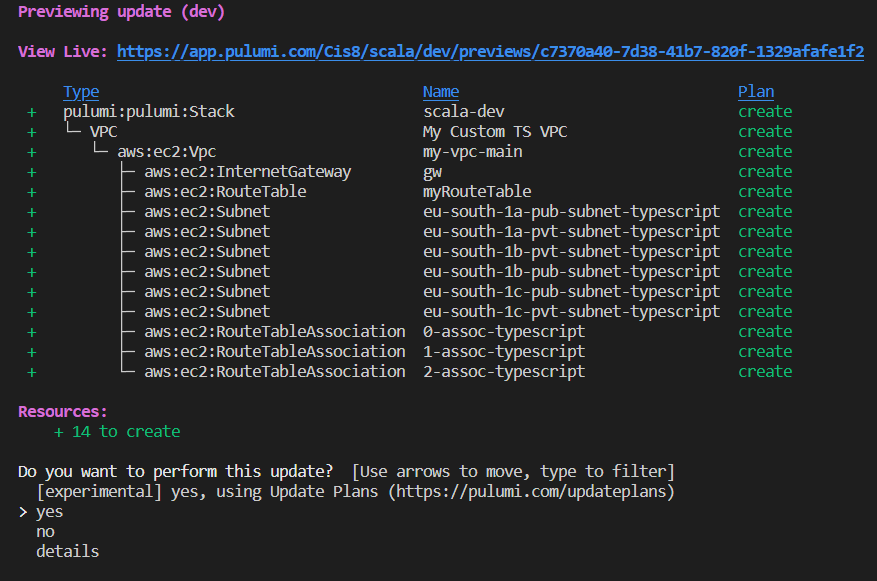
\includegraphics[width=1\columnwidth]{case_study/pulumi_up_1} 
  \captionof{figure}{pulumi up preview}
\end{center}\mbox{}\\

If we press yes this is the output:
\begin{center}
  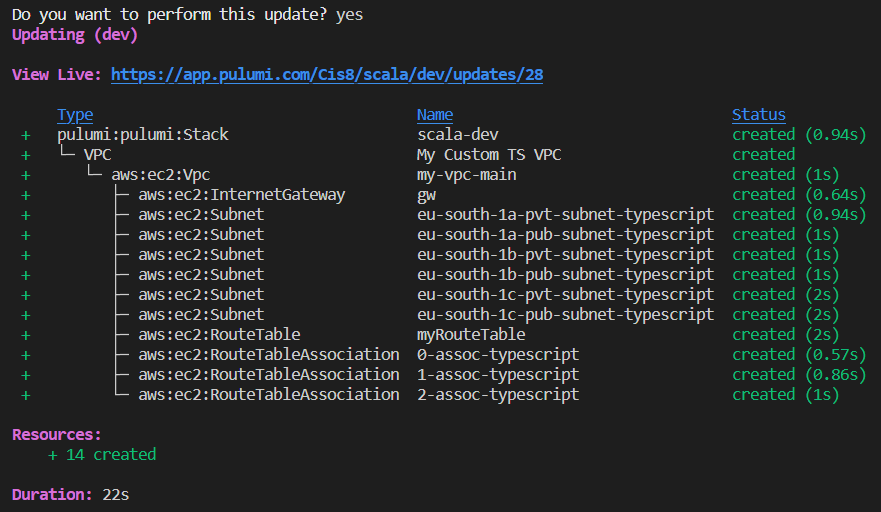
\includegraphics[width=1\columnwidth]{case_study/pulumi_up_2} 
  \captionof{figure}{pulumi up confirmed}
\end{center}\mbox{}\\
We can notice how the resources created are nested into each other thanks to the parent option that we used.
This is helping us in keeping our resources on the stuck nicely ordered and tied up.\\

\section{Destroying the resources with Pulumi}
Now lets use the \texttt{pulumi destroy} command to destroy the resources on our Pulumi's stack.
The preview of the changes that we are about to get look like this:
\begin{center}
  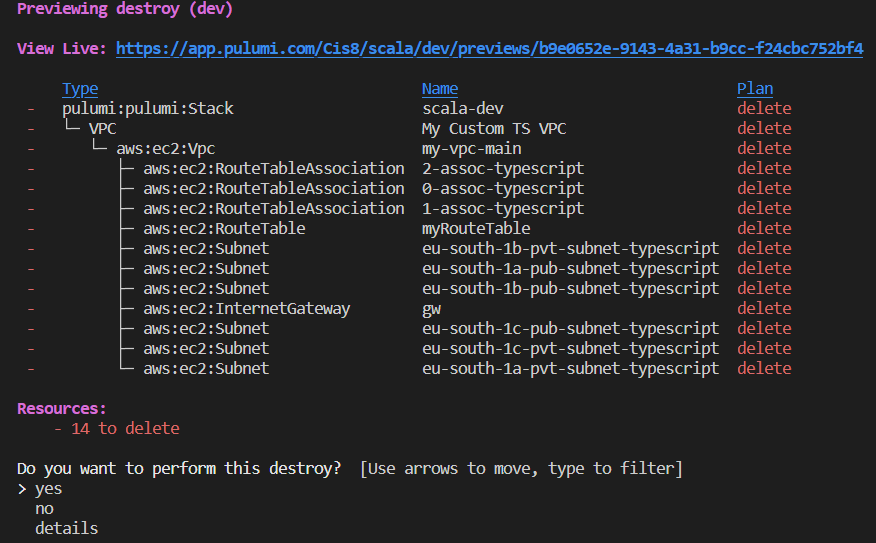
\includegraphics[width=1\columnwidth]{case_study/pulumi_destroy_1} 
  \captionof{figure}{pulumi destroy preview}
\end{center}\mbox{}\\

If we confirm the changes this is the result:
\begin{center}
  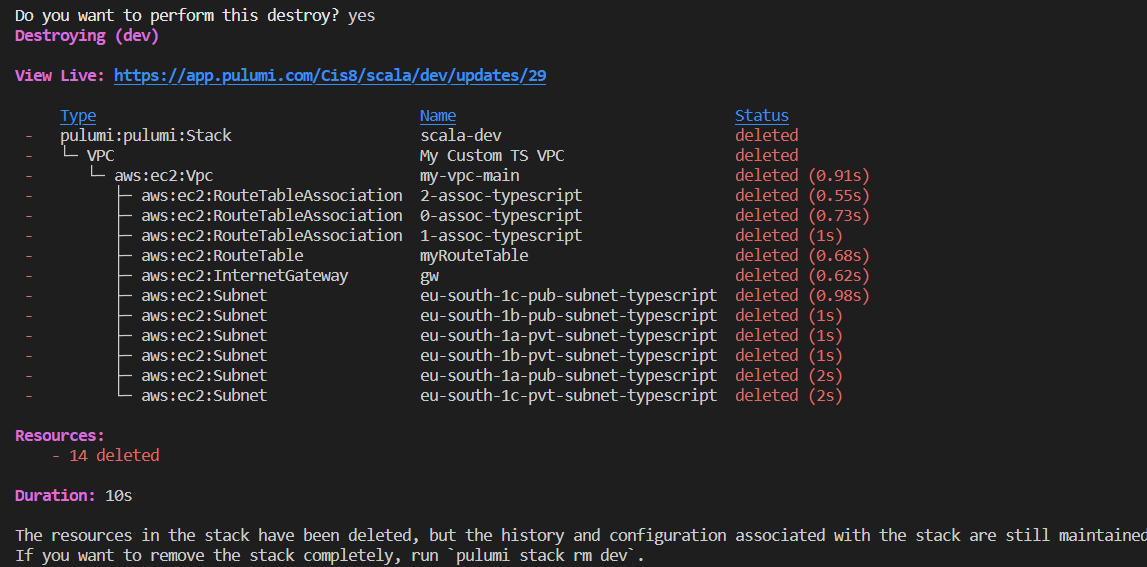
\includegraphics[width=1\columnwidth]{case_study/pulumi_destroy_2} 
  \captionof{figure}{pulumi destroy confirmed}
\end{center}\mbox{}\\

%\section{Java implementation of the case study}

\section{My Scala implementation of the case study}
Since Scala is not supported by Pulumi, I had to implement it on my own.
The Pulumi team is clear on the official way to add the support of a new language for Pulumi, and the procedure is long and laborious, too laborious for a master thesis.
The full procedure can be found on \href{https://github.com/pulumi/pulumi/wiki/New-Language-Bring-up}{New Language Bring Up}.\\
The idea behind the adopted solution is to exploit the compatibility of Scala with the Java libraries to write custom syntactic sugar.
Such syntactic sugar will be based on the Pulumi Java's APIs and will provide to the user cool constructs to write readable and expressive code to interact with Pulumi.\\
The steps of the work done have been the followings:
\begin{enumerate}
  \item manually write the \textit{sugarized} functions to create the Pulumi resources using Scala
  \item use such functions to recreate the Stack obtained with the typescript solution shown before in the \hyperref[sec:typescript-impl]{Typescript implementation of the case study} section
  \item create an automatic code generator for our syntactic sugar functions, so that we can quickly create a library for Scala's Pulumi APIs
  \item try to recreate the stack with the automatically generated code
\end{enumerate}
Obviously, the third step is quite wide, and if fact with my work I had the time to generate only the functions for a part of the Java's Pulumi APIs for the AWS EC2 module.\\
Now the just defined steps will more accurately presented.

\subsection{Structure of the Java APIs for the constructors of the resources in Pulumi}
To understand the syntactic sugar functions that I defined, let's first consider the general structure of the Java APIs for the constructors of the resources.\\
The constructor of a resource, in general accepts a name and an instance of the corresponding \texttt{Args} class of the resource we are creating.
Lets consider for example the Vpc resource.
In Java, to instantiate such a resource we'd call:
\begin{lstlisting}[numbers=left, numberstyle=\tiny, numbersep=-5pt, stepnumber=1]
  protected Vpc vpc = new Vpc("my-vpc-java", VpcArgs.builder()
    .cidrBlock("10.136.0.0/24")
    .tags(Map.of("Name", "main"))
    .build(),
          CustomResourceOptions.builder()
                  .parent(this)
                  .build());
\end{lstlisting}\mbox{}\\
We can (hardly) see that along with the name to be assigned to the vpc "my-vpc-java", a VpcArgs builder and a CustomResourceOptions builder are passed by.
These builders will create an instance of the respective classes that will be used to set respectively the parameters and the parent of the Vpc resource.
So, for our case study we need to consider: the name to be assigned at the created resource on the Pulumi stack, the builder of the respective \texttt{Args} class of the resource, and the \texttt{CustomResourceOptions} builder.


\subsection{Syntactic sugar}
Our syntactic sugar is split in 2 categories of functions.
The first is about the functions that represent the constructors of the resources.
The second is for the methods available within the builders of the \texttt{Args} classes and for the CustomResourceOptions builder functions.
The idea to create a resource is to call the \textit{sugarized} function that represent the constructor of that resource, and and then call the Builder methods to assign the various parameters to the resource.

\subsubsection{Vpc creation}
This is how a Vpc resource can be created with my syntactic sugar:
\begin{lstlisting}[numbers=left, numberstyle=\tiny, numbersep=-5pt, stepnumber=1]
  val myVpc: Vpc = vpc("scala-main") ({
    cidrBlock("10.136.0.0/24")
    tags("Name" -> "myVpcScala")
  },{
    parent(this)
  })
\end{lstlisting}\mbox{}\\
At line 1, the \texttt{vpc} function is the actual \textit{sugarized} function for the VPC resource constructor.
In fact we can notice that we have a curried function.
The first parenthesis is taking the parameter for the resource name on the Pulumi stack, while the second one is containing two lambdas (defined by the curly brackets).
These lambdas are respectively used to call all the builder methods of the \texttt{VcpArgs} class and the ones for the \texttt{CustomResourceOptions}.\\
We can notice that we didn't explicitly defined an instance of the builders of such classes.
We will soon see how we achieved such a syntactic sugar trick.\\
The \texttt{cidrBlock} and the \texttt{tags} methods are the generated methods for builder of the \texttt{VpcArgs} class.\\ 
The \texttt{parent} method instead is the generated method for the builder of the \texttt{CustomResourceOptions} class.\\
Moreover, we can also notice that inside tags, that expects a \texttt{Map[String, String]} type, the instantiation of a \texttt{Map[String, String]} containing a single elements isn't required.
This other trick will be explained later as well.

\subsubsection{Internet gateway creation}
Much similar to the VPC resource, we have this code for the internet gateway creation:
\begin{lstlisting}[numbers=left, numberstyle=\tiny, numbersep=-5pt, stepnumber=1]
  val myIGW: InternetGateway = internetGateway("gw") ({
    vpcId(myVpc.getId())
    tags("Name" -> "myIGWScala")
  },{
    parent(myVpc)
  })
\end{lstlisting}\mbox{}\\
The code won't be commented since is analogous to the VPC case.

\subsubsection{Routing table creation}
The code to create a routing table:
\begin{lstlisting}[numbers=left, numberstyle=\tiny, numbersep=-5pt, stepnumber=1]
  val myRouteTable = routeTable("myRouteTable") ({
    vpcId(myVpc.getId())
    routes(
      routeTableRouteArgs(){
        cidrBlock("0.0.0.0/0")
        gatewayId(myIGW.getId())
      })
    tags("Name" -> "myRouteTableScala")
  },{
    parent(myVpc)
  })
\end{lstlisting}\mbox{}\\
The only thing that is worth to mention here is that the \texttt{routes} function, at line 3, expects a \texttt{List[RouteTableRouteArgs]}, but we are providing only a \texttt{RouteTableRouteArgs}.
As for the case of the \texttt{Map[String, String]} with the parent method mentioned above, the same trick has been used to provide syntactic sugar that lifts us from the need of instantiate a singleton \texttt{List[RouteTableRouteArgs]} manually.

\subsubsection{Subnets creation}
Much different from the other resources is the function to create the subnets:
\begin{lstlisting}[numbers=left, numberstyle=\tiny, numbersep=-5pt, stepnumber=1,linewidth=420pt]
  def createAzSubnets(isPvt: Boolean) =
    availabilityZonesNames().map((az: GetAvailabilityZonesResult) =>
      for
        (name, cidr) <- az.names().zip(if isPvt then pvtSubnetsCidrs else pubSubnetsCidrs)
      yield
        val compName = name + "-" + (if isPvt then "pvt" else "pub") + "-subnet-scala"
        subnet(compName) ({
          vpcId(myVpc.getId())
          availabilityZone(name)
          cidrBlock(cidr)
          tags("Name" -> compName)
        },{
          parent(myVpc)
        })
    )
\end{lstlisting}\mbox{}\\


\subsubsection{Syntactic sugar for the builders}


\subsubsection{Syntactic sugar for the constructors of the resources}

\subsubsection{Functor and Monads for the Output type}

\subsection{Automatic code generation for the syntactic sugar}

\subsubsection{What Pulumi asks for the official support of a new Language}

\subsubsection{Raw automatic code generation with JavaParser}

\subsubsection{Usage of the generated code as a library}

\subsubsection{Possible future improvements for the code generation with Scalameta}
